\documentclass{article}
\usepackage[utf8]{inputenc}
\usepackage{fancyhdr}
\usepackage{graphicx}

% ---- Commands ------- %
\newcommand{\documentNumber}[1]{
    \LARGE  \textbf{ PUSP2142{#1} } \\
    \medskip
}
\newcommand{\documentVersion}[1]{
    v.{#1} \\
    \medskip
}
\newcommand{\documentTitle}[1]{
    \centerline{\rule{13cm}{0.4pt}}
    \bigskip \bigskip
    \LARGE {#1} \\
    \bigskip \bigskip
    \centerline{\rule{13cm}{0.4pt}}
}
\newcommand{\documentGroup}[1]{
    \bigskip \bigskip
    \LARGE Group {#1} \\
    \bigskip
}
\newcommand{\documentResponsible}[1]{
    \LARGE Responsible: {#1} \\
    \medskip
}
\newcommand{\documentAuthors}[1]{
    \LARGE Authors: {#1} \\
    \medskip    
}
\newcommand{\documentDate}[1]{
    \date {#1} 
}

\graphicspath{{./images/}} %Defines a path to file images

% --- Header & Footer ---- %
\pagestyle{fancy}
\lhead{\leftmark}
\rhead{}
\rfoot{\thepage}
\cfoot{}
\lfoot{}


% ------------------------------------------------ #

% ----- FILL THIS ----- %
\title {
    % Must be 2 digits
    \documentNumber {01}    
    
    \documentVersion {0.1}
    
    % Full name - SHORTNAME
    \documentTitle {\LaTeX \hspace{} Lazy dog}
    \documentGroup {2}
    
    % Options: - Project management Group
    %          - System architecture Group
    %          - Developer Group
    %          - Test Group
    \documentResponsible {Project management Group}
    \documentAuthors {System architecture Group, Development Group}
    
    % Format: YYYY-MM-DD
    \documentDate {2021-01-25}
}

\begin{document}

\maketitle
\thispagestyle{empty}

\newpage

\tableofcontents

\newpage

%---------Document begins here-----------

\section{This is a section}
    This document is meant to be read side by side with the source code. 
    \subsection{This is a subsection}
        It wont make a lot of sense otherwise. 
        \subsubsection{This is a subsubsection}
            Please feel free to look at the source code if you get stuck. 
            
\section{Useful formating tools}
    Latex supports lists, there are many variations of lists so if this format doesnt suit you google is your friend. 
    
    Heres a list of useful formating tools. 
    \begin{itemize}
        \item \textbackslash newline %Since backslashes are used to denote commands there naturally has to be a backslash preceeded command for backslashes
        \item \textbackslash newpage
    \end{itemize}
    
    You can also make ordered lists. This list ranks the project managers by latex their skills
    
    \begin{enumerate}
        \item Assar Orpana
        \item Victor Krook
    \end{enumerate}
    
    Since I dont want the next page to be interrupted by a page break, I will now use the \textbackslash newpage command to force a page break. 
    \newpage
    
\section{Tables and images}
    \subsection{How tables works}
        Latex has built in table support. It looks a bit daunting but it's quite easy.
        
        The tabular environmet is wrapped in a table environment to support captions and centering. The [h] argument stands for "here", meaning that the table is rendered at the location that it occurs in the .tex file. 
        \begin{table}[h] %The table environment is used for captions and forcing placement
            \centering
            \begin{tabular}{|c|c|c|c|} %The pipe symbols tell the compiler where the vertical lines go. The numbers of c's decide how many columns the table has.
            \hline %The hline command inserts a horizontal line
                 (0, 0) & (1, 0) & (2, 0) & (3, 0) \\ %Cells are seperated horizontaly by the & symbol.
            \hline            
                 (0, 1) & (1, 1) & (2, 1) & (3, 1) \\ %Double backslashes jumps to the next row
            \hline
            \end{tabular} %Remember that everything with a begining has an end
            \caption{This is a caption} %This line adds a caption to the table
        \end{table}
        
        \subsection{Pictures}
        Latex also supports images. Simply use the includegraphics environment. Every document folder should include a subfolder named "images" where images are stored. The path to the images folder is defined at the top of the .tex file. 
        
        Use the figure environment for adding captions and forcing placement when adding images to your document. Just as with the table, use an [h] tag to force placement. Use the \textbackslash centering command to center tables and figures. 
        
        Figures can also be used as references. Figure \ref{bigdog} is larger than figure \ref{smalldog}
        
        \LaTeX \hspace{} does not concern itself with formating images. You should therefore know the scale argument. 
        \begin{figure}[h]
            \centering
            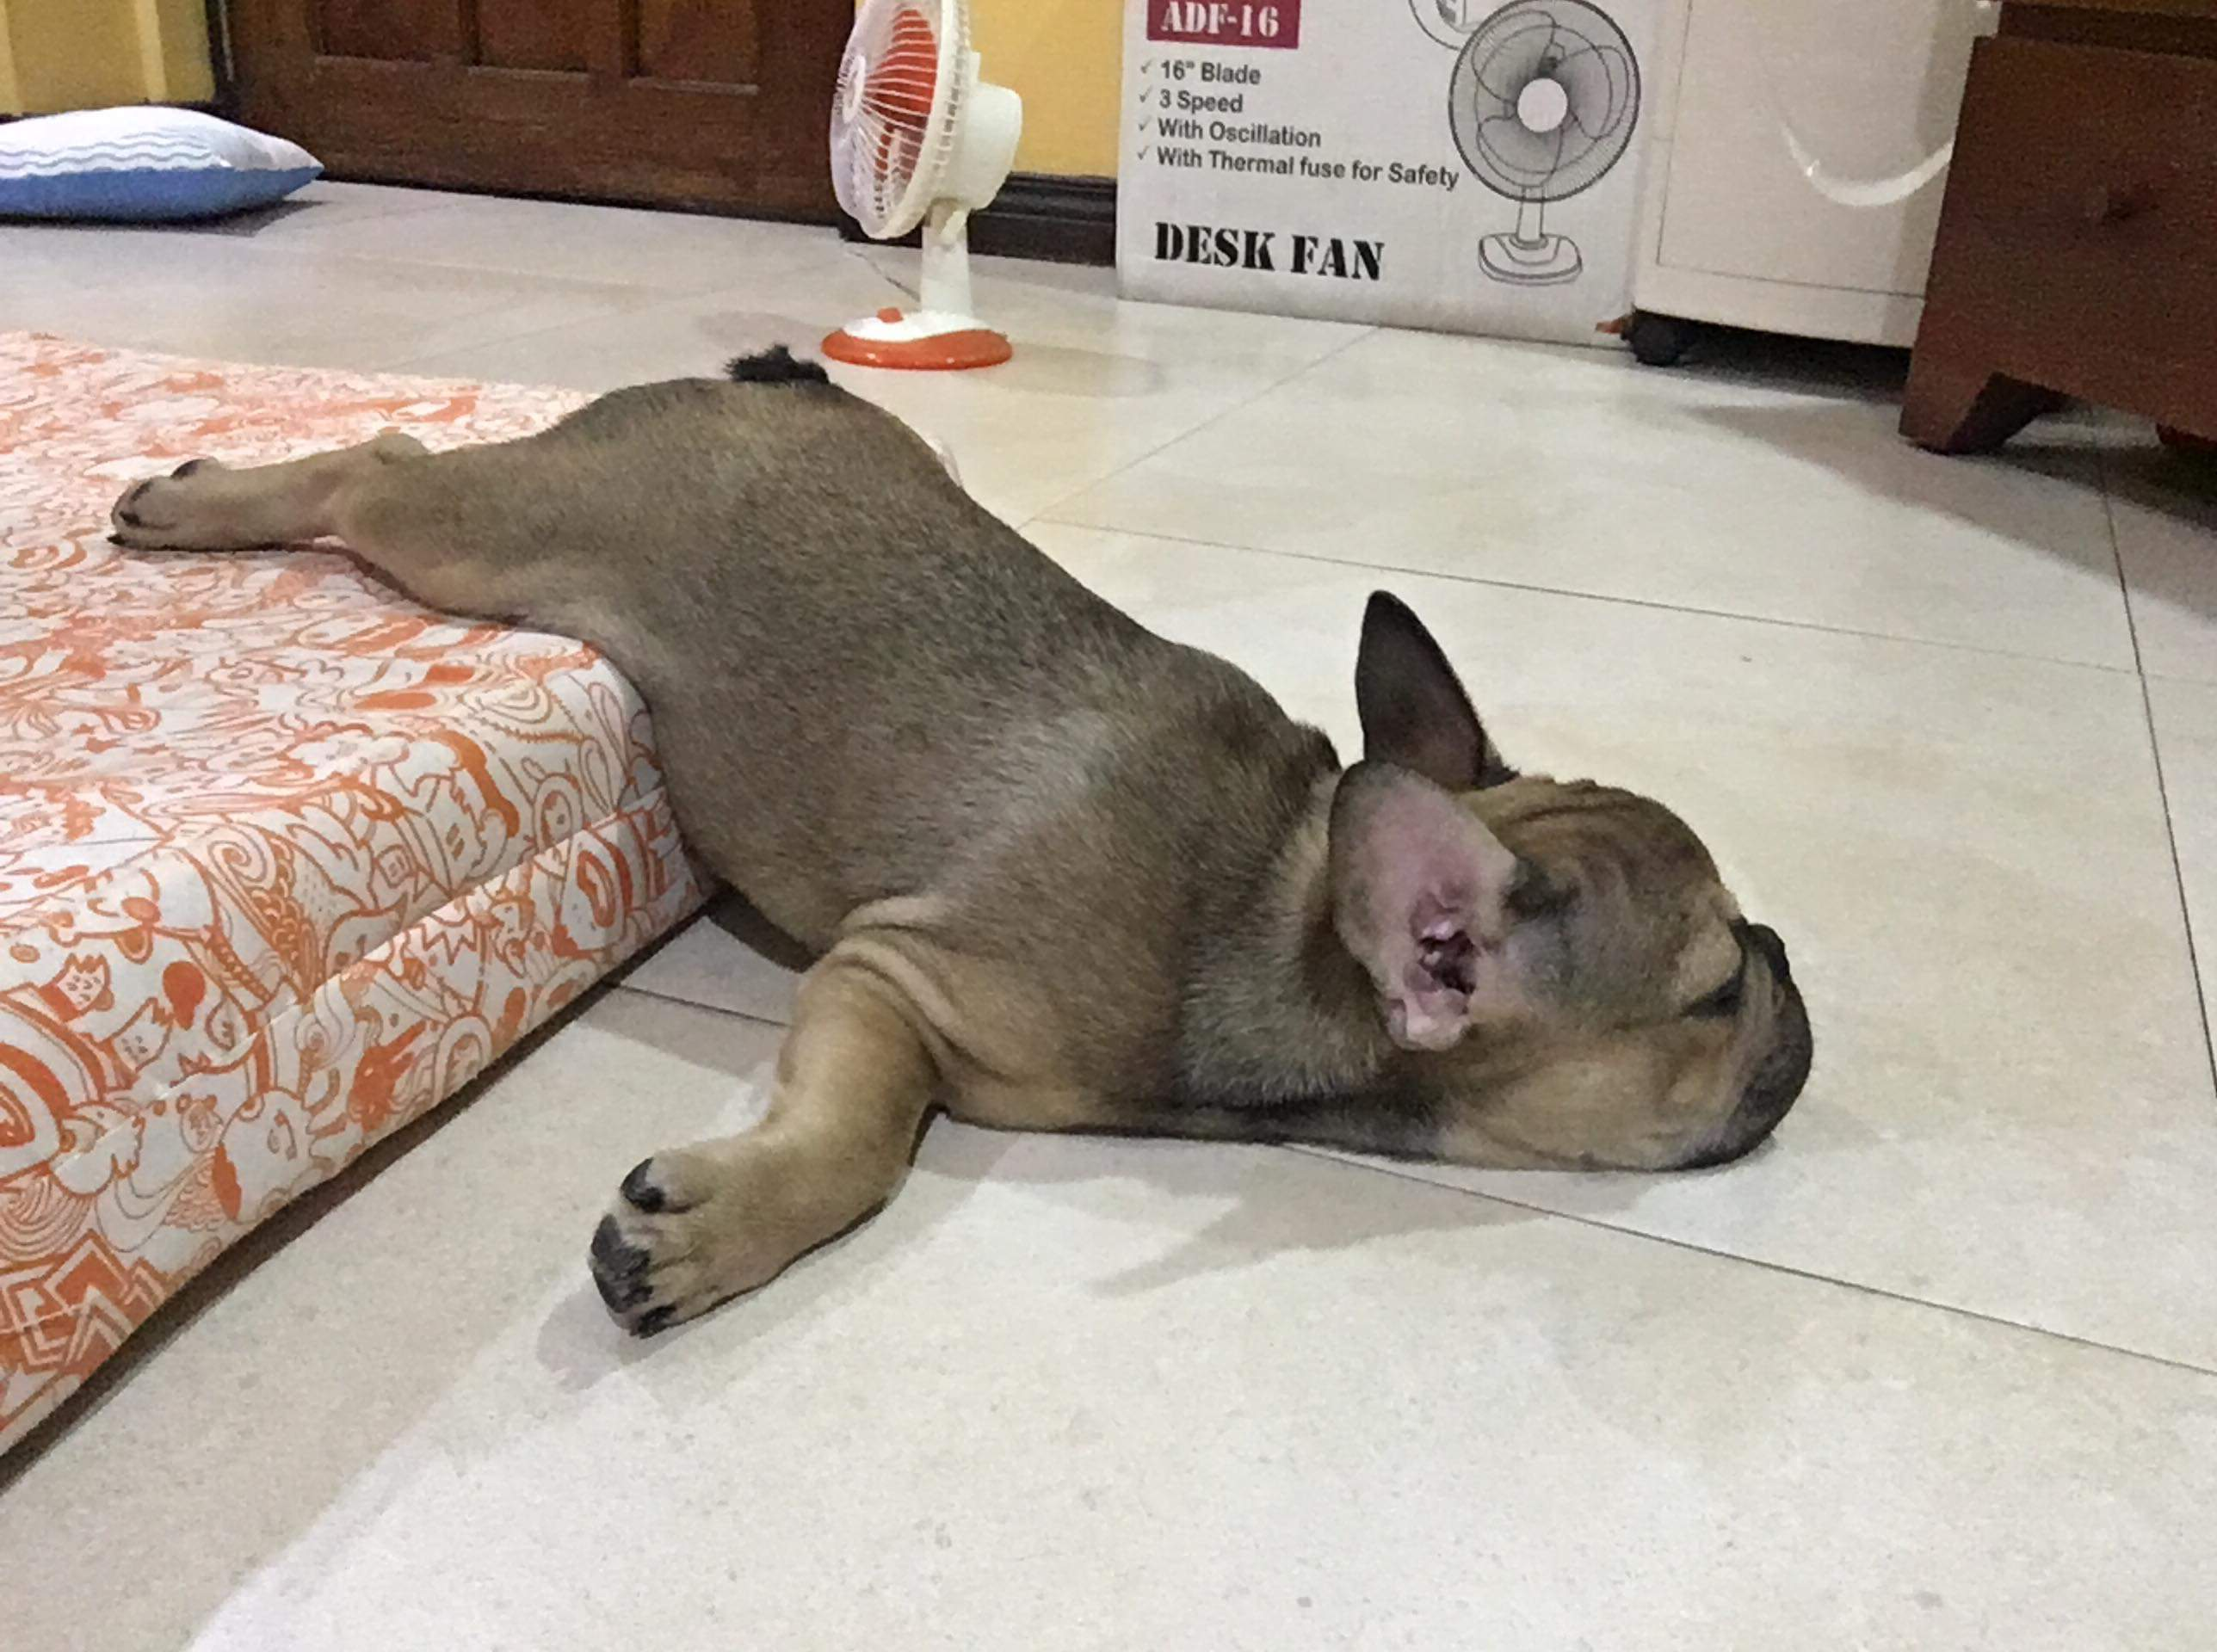
\includegraphics[scale=0.01]{dog} %This is the line that inserts the image, the scale argument affects the size of the image and "dog" is the name of the image in the images folder. The location of the images folder is defined at the top of the document. 
            \caption{A cute dog at scale=0.02, with centering}
            \label{smalldog} %Labels are used for making references. They are useful when you want to add an image without having to redo all your captions. 
        \end{figure}
        
        \begin{figure}[h]
            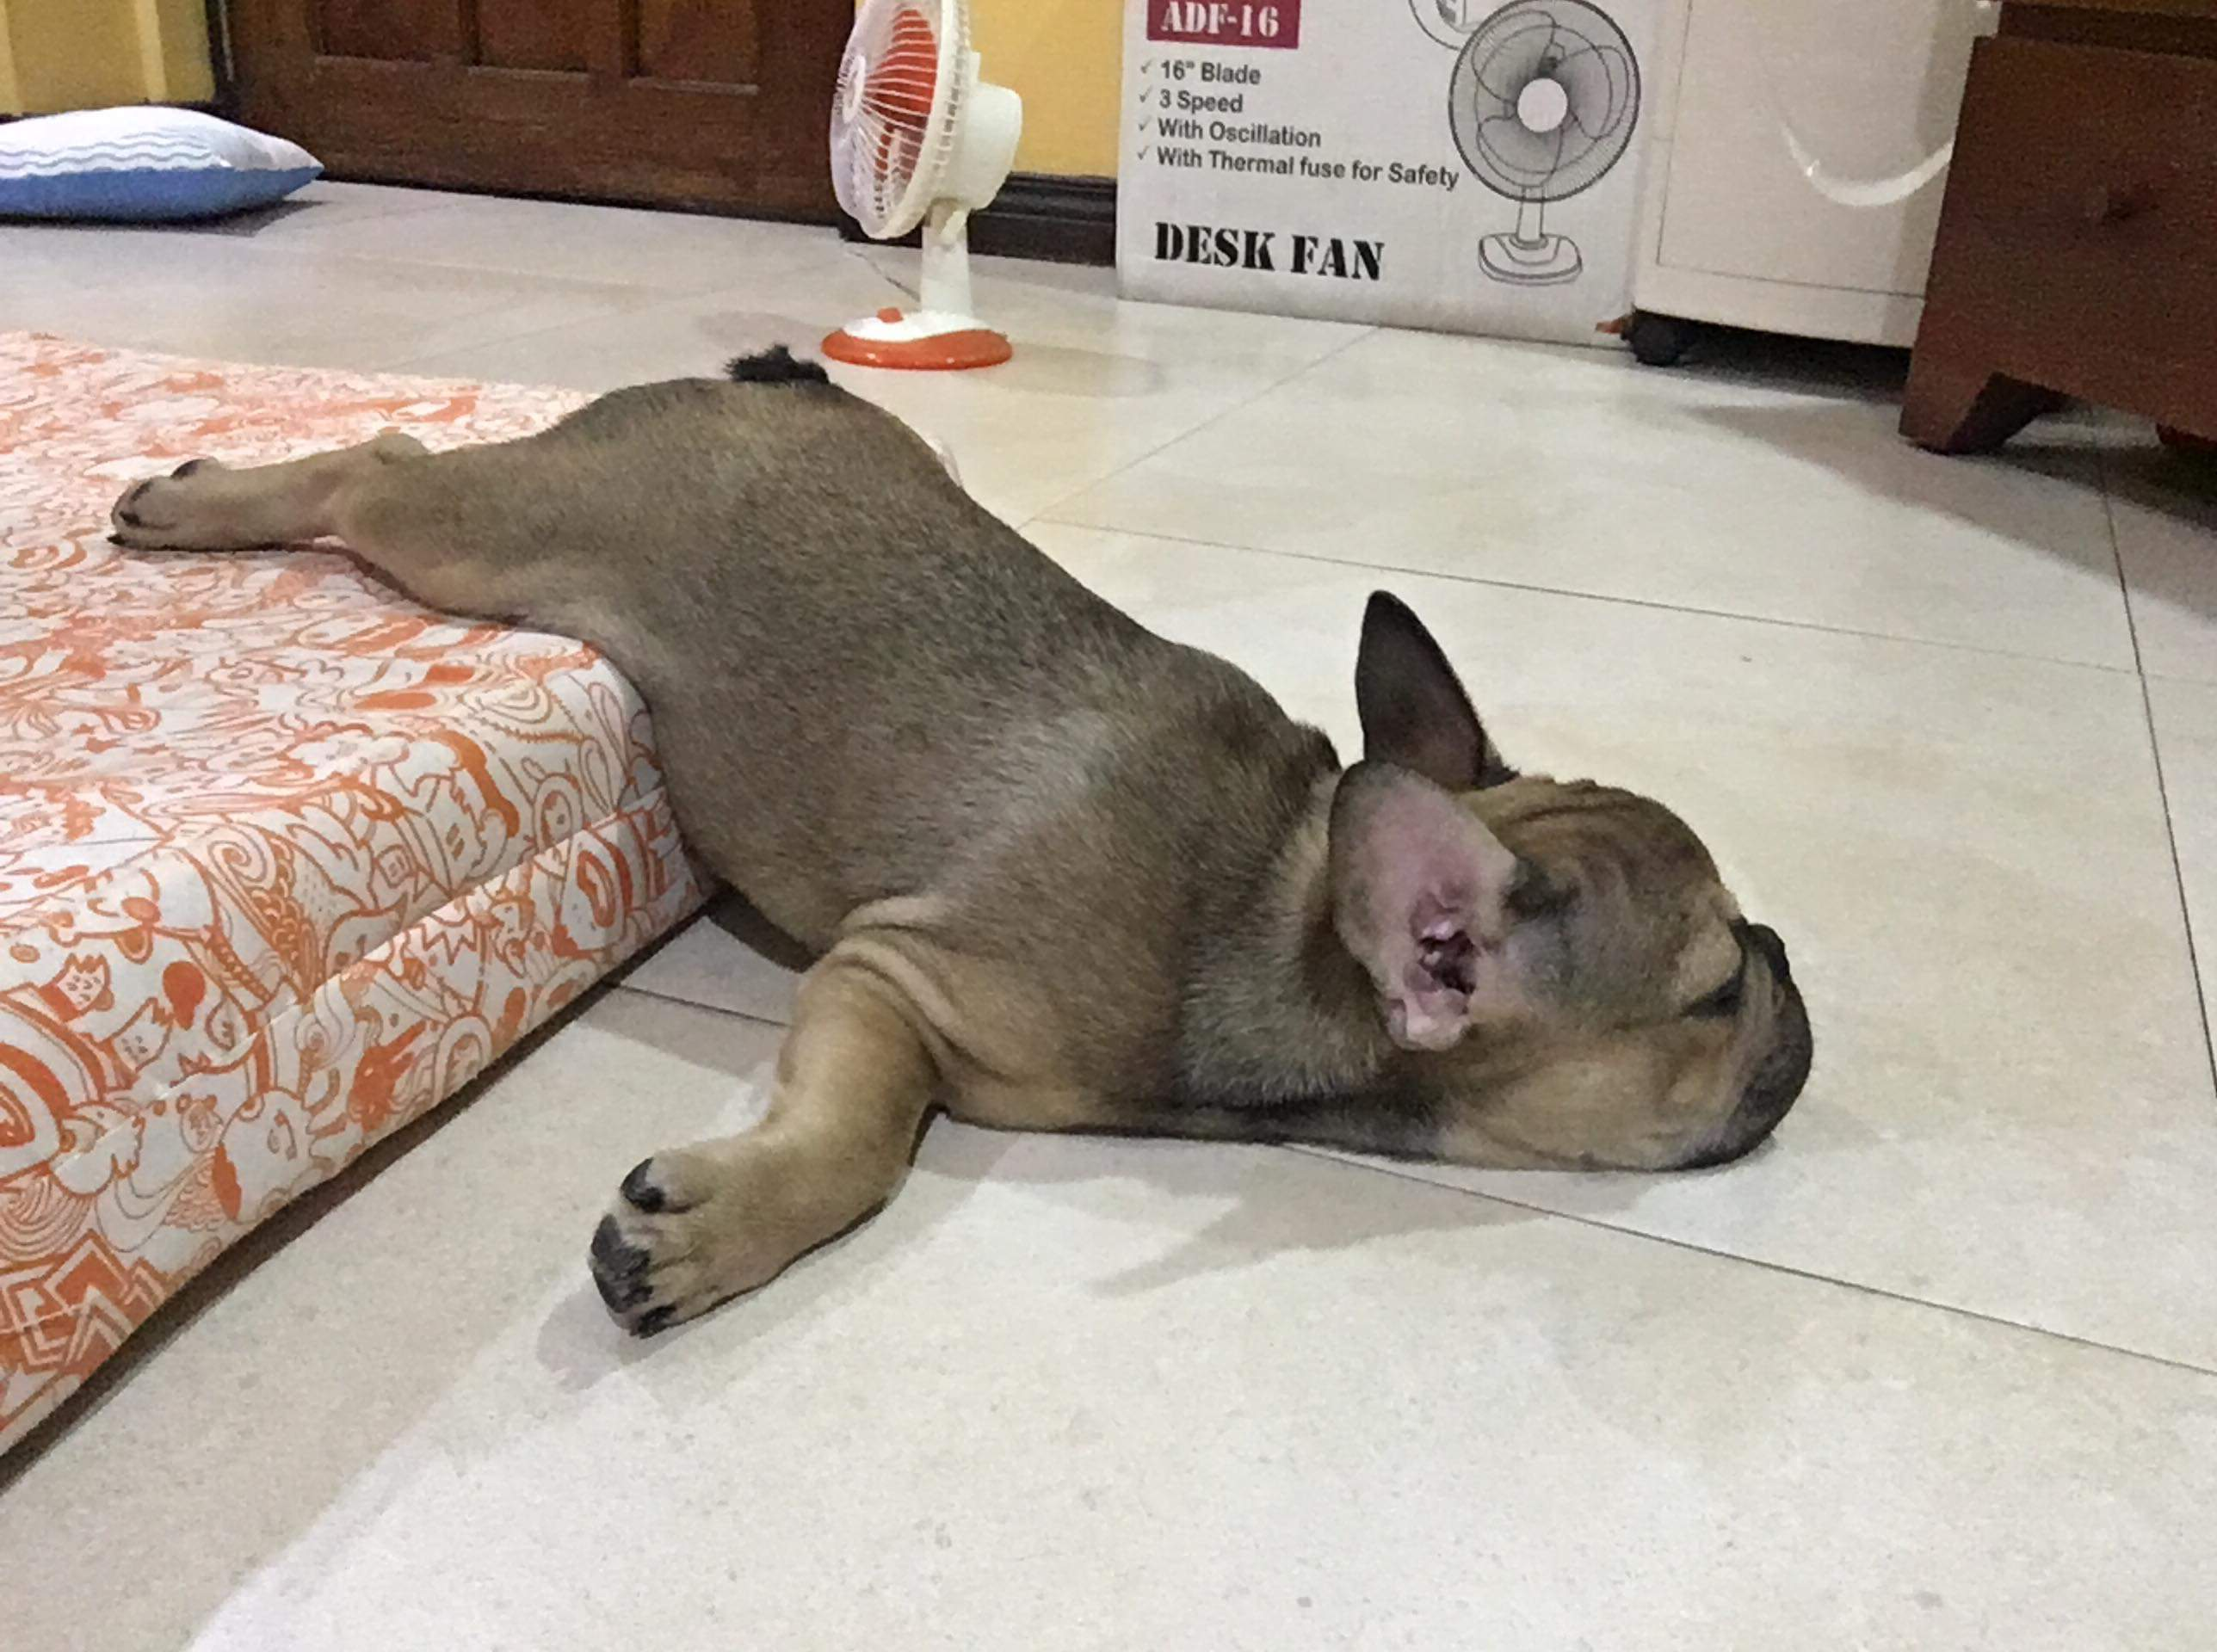
\includegraphics[scale=0.04]{dog}
            \caption{A cute dog at scale=0.04, without centering}
            \label{bigdog}
        \end{figure}

\end{document}
